\documentclass{article}
\usepackage{fontspec}
\setmainfont[Mapping=tex-text]{CMU Serif}
\setsansfont[Mapping=tex-text]{CMU Sans Serif}
\setmonofont{CMU Typewriter Text}
\usepackage{graphicx}
\usepackage{enumitem}
\usepackage{fixltx2e}
\usepackage{array,booktabs,arydshln,xcolor}
\newcommand\VRule[1][\arrayrulewidth]{\vrule width #1}
\usepackage{amsthm}
\usepackage{amsmath}
\usepackage{amssymb}
\usepackage[ruled,vlined]{algorithm2e}
\usepackage{nccmath}
\usepackage{multirow}
\usepackage[left=3cm,right=3cm]{geometry}
\usepackage{csquotes}
\usepackage{diagbox}
\usepackage{float}
\usepackage{tikz}
\usepackage{tkz-graph}
\renewcommand*{\EdgeLineWidth}{0.15pt}
\usepackage{listings}
\renewcommand{\refname}{Αναφορές}
\tikzset{LabelStyle/.style= {draw,
fill = white,
text = black}}
\definecolor{mGreen}{rgb}{0,0.6,0}
\definecolor{mGray}{rgb}{0.5,0.5,0.5}
\definecolor{mPurple}{rgb}{0.58,0,0.82}
\definecolor{backgroundColour}{rgb}{0.95,0.95,0.92}

\lstdefinestyle{CStyle}{
    backgroundcolor=\color{backgroundColour},   
    commentstyle=\color{mGreen},
    keywordstyle=\color{magenta},
    numberstyle=\tiny\color{mGray},
    stringstyle=\color{mPurple},
    basicstyle=\footnotesize,
    breakatwhitespace=false,         
    breaklines=true,                 
    captionpos=b,                    
    keepspaces=true,                 
    numbers=left,                    
    numbersep=5pt,                  
    showspaces=false,                
    showstringspaces=false,
    showtabs=false,                  
    tabsize=4,
    language=C
}

\makeatletter
\newenvironment{chapquote}[2][2em]
  {\setlength{\@tempdima}{#1}%
   \def\chapquote@author{#2}%
   \parshape 1 \@tempdima \dimexpr\textwidth-2\@tempdima\relax%
   \itshape}
  {\par\normalfont\hfill--\ \chapquote@author\hspace*{\@tempdima}\par\bigskip}
\makeatother

\title{{\includegraphics[scale=0.2]{./photos/pyrforos.jpg} \\ \vspace{15mm}  \textbf{ΣΥΣΤΗΜΑΤΑ ΠΑΡΑΛΛΗΛΗΣ ΕΠΕΞΕΡΓΑΣΙΑΣ}} \vspace{5mm} \\ Άσκηση 1: Παραλληλοποίηση αλγορίθμων σε πολυπύρηνες αρχιτεκτονικές κοινής μνήμης  \vspace{5mm} \\ \small Χειμερινό εξάμηνο 2019-20 - Ροή Υ}

\author{
  Αντωνιάδης, Παναγιώτης\\
  \texttt{el15009@central.ntua.gr}
  \and
  Μπαζώτης, Νικόλαος\\
  \texttt{el15739@central.ntua.gr}
}

\date{\hrule}


\begin{document}

\maketitle

\begin{chapquote}{ Gene Amdahl, \textit{American computer architect}}
``For over a decade prophets have voiced the contention that the organization of a single computer has reached its limits and that truly significant advances can be made only by interconnection of a multiplicity of computers.''
\end{chapquote}

\pagebreak


\section{Conway's Game of Life}

\subsection{Σκοπός της ενότητας}

Σκοπός της συγκεκριμένης ενότητας της άσκησης είναι η εξοικείωση με τις υποδομές του εργαστηρίου (πρόσβαση στα συστήματα, μεταγλώττιση προγραμμάτων, υποβολή εργασιών κλπ) μέσα από την παραλληλοποίηση ενός απλού προβλήματος σε αρχιτεκτονικές κοινής μνήμης.


\subsection{Περιγραφή}

Το Παιχνίδι της Ζωής (Conway's Game of Life) λαμβάνει χώρα σε ένα ταμπλό με κελιά δύο διαστάσεων. Το περιεχόμενο κάθε κελιού μπορεί να είναι γεμάτο (alive) ή κενό (dead), αντικατοπτρίζοντας την ύπαρξη ή όχι ζωντανού οργανισμού σε αυτό, και μπορεί να μεταβεί από τη μία κατάσταση
στην άλλη μία φορά εντός συγκεκριμένου χρονικού διαστήματος. Σε κάθε βήμα (χρονικό διάστημα),
κάθε κελί εξετάζει την κατάστασή του και αυτή των γειτόνων του (δεξιά, αριστερά, πάνω, κάτω και
διαγώνια) και ακολουθεί τους παρακάτω κανόνες για να ενημερώσει την κατάστασή του:

\begin{itemize}
\item Αν ένα κελί είναι ζωντανό και έχει λιγότερους από 2 γείτονες πεθαίνει από μοναξιά.
\item Αν ένα κελί είναι ζωντανό και έχει περισσότερους από 3 γείτονες πεθαίνει λόγω υπερπληθυσμού.
\item Αν ένα κελί είναι ζωντανό και έχει 2 ή 3 γείτονες επιβιώνει μέχρι την επόμενη γενιά.
\item Αν ένα κελί είναι νεκρό και έχει ακριβώς 3 γείτονες γίνεται ζωντανό (λόγω αναπαραγωγής).
\end{itemize}


\subsection{Υλοποίηση}

Παρακάτω παρατίθεται η κύρια επανάληψη της σειριακής υλοποίησης που μας δίνεται:

\begin{lstlisting}[style=CStyle]
for ( t = 0 ; t < T ; t++ ) {
	for ( i = 1 ; i < N-1 ; i++ ){
    	for ( j = 1 ; j < N-1 ; j++ ) {
    		// Compute number of neighbors
        	nbrs = previous[i+1][j+1] + previous[i+1][j] + previous[i+1][j-1] \
                     + previous[i][j-1] + previous[i][j+1] \
                     + previous[i-1][j-1] + previous[i-1][j] + previous[i-1][j+1];
            if ( nbrs == 3 || ( previous[i][j]+nbrs ==3 ) )
            	// Cell is alive
            	current[i][j]=1;
            else
            	// Cell is dead
                current[i][j]=0;
           	}
	}
	// Swap current array with previous array
    swap=current;
    current=previous;
    previous=swap;
}
\end{lstlisting}

Αφού μετά από κάθε χρονική στιγμή ανανεώνουμε όλο το ταμπλό δεν μπορούμε να παραλληλοποιήσουμε την διαδικασία ως προς τις χρονικές στιγμές. Όμως, το γεγονός ότι η ανανέωση ενός κελιού εξαρτάται μόνο από τα γειτονικά του μας δίνει την δυνατότητα να παραλληλοποιήσουμε την διαδιακασία της ανανέωσης του N×N πίνακα. Χρησιμοποώντας το OpenMP, προσθέτουμε στην γραμμή 2 την εξής εντολή:

\begin{lstlisting}[style=CStyle]
#pragma omp parallel for shared(N, previous, current) private(i, j, nbrs)
\end{lstlisting}

με η οποία ουσιαστικά ζητάμε να παραλληλοποιηθούν οι εσωτερικοί βρόγχοι με όσα νήματα έχουν οριστεί (μεταβλητή περιβάλλοντος OMP\_NUM\_THREADS). Οι μεταβλητή N και οι δύο δείκτες μοιράζονται από τα νήματα ενώ οι μεταβλητές i, j, nbrs είναι ατομικές για το κάθε νήμα.

\subsection{Αποτελέσματα}

Όλες οι μετρήσεις για το Game of Life πραγματοποιήθηκαν για 1000 γενιές. Οι παράμετροι οι οποίοι μεταβάλλαμε κάθε φορά ήταν το μέγεθος του ταμπλό και ο αριθμός των πυρήνων και όλοι οι συνδυασμοί συνοψίζονται στον παρακάτω πίνακα (χρόνος σε second):

\begin{center}
 \begin{tabular}{|c|*{3}{c|}}
 \hline
  \diagbox{Cores}{Table Size}&  64×64 & 1024×1024 & 4096×4096 \\ \hline
 1 & 0.023186 & 10.962964 & 175.840471 \\
 \hline
  2 & 0.013763 & 5.455029 & 88.314822 \\
 \hline
 4 & 0.010027 & 2.722563 & 44.508848 \\
 \hline
 6 & 0.009616 & 1.830053 & 36.922346 \\
 \hline
 8 & 0.010151 & 1.377850 & 36.343052 \\
 \hline
\end{tabular}
\end{center}

Για να ερμηνεύσουμε τα παραπάνω αποτελέσματα, κατασκευάσαμε για κάθε μέγεθος ταμπλό δύο διαγράμματα όπου παριστάνουν την μεταβολή του χρόνου και του speedup καθώς αυξάνεται ο αριθμός των πυρήνων. Να σημειωθεί ότι ως speedup ορίζεται ο λόγος του χρόνου του σειριακού προγράμματος προς τον χρόνο του παράλληλου ($S = \frac{T_s}{T_p}$). Να σημειωθεί, ότι προφανώς αυτό που επιδιώκουμε όταν παραλληλοποιούμε ένα πρόγραμμα είναι να μειώσουμε τον χρόνο εκτέλεσης. Ιδανικά, θέλουμε η προσθήκη περισσότερων πυρήνων να μειώνει με ανάλογο τρόπο τον χρόνο εκτέλεσης του προγράμματος και ώστε $S = p$. Ωστόσο, αυτό δεν συμβαίνει διότι τα νήματα κάποια στιγμή θα επικοινωνήσουν για να ανταλλάξουν δεδομένα, όπως επίσης, η δημιουργία και ο τερματισμός των νημάτων απαιτεί κάποιο χρόνο που σε ένα σειριακό πρόγραμμα δεν θα χρειαζόταν.

\pagebreak 

\begin{itemize}
\item \textbf{64×64}

\begin{figure}[H]
  \centering
    \includegraphics[width=0.6\textwidth]{../ex1/plots/table_size/time/time_64.png}
\end{figure}

\begin{figure}[H]
  \centering
    \includegraphics[width=0.6\textwidth]{../ex1/plots/table_size/speedup/speedup_64.png}
\end{figure}


\textbf{Σχολιασμός:}
Η μείωση του χρόνου δεν αυξάνεται ανάλογα με τον αριθμό των πυρήνων. Ειδικότερα, για 4 και 6 πυρήνες έχουμε ελάχιστη μείωση ενώ για 8 πυρήνες ο χρόνος εκτέλεσης αυξάνεται. Αυτό συμβαίνει, διότι το ταμπλό είναι μικρό και ο συνολικός χρόνος εκτέλεσης ακόμα και του σειριακού προγράμματος είναι μικρός. Έτσι, από ένα σημείο και μετά η δημιουργία των νημάτων και η επικοινωνία μεταξύ τους για την ανταλλαγή δεδομένων σπαταλά περισσότερο χρόνο από αυτόν που κερδίζουμε εκτελώντας το πρόγραμμα παράλληλα.


\item \textbf{1024×1024}

\begin{figure}[H]
  \centering
    \includegraphics[width=0.6\textwidth]{../ex1/plots/table_size/time/time_1024.png}
\end{figure}

\begin{figure}[H]
  \centering
    \includegraphics[width=0.6\textwidth]{../ex1/plots/table_size/speedup/speedup_1024.png}
\end{figure}

\textbf{Σχολιασμός:} Παρατηρούμε ότι το 1024×1024 ταμπλό αποτελεί μία πολύ καλή περίπτωση παραλληλισμού. Καθώς αυξάνουμε τον αριθμό των πυρήνων ο χρόνος πέφτει στο μισό και το speedup διπλασιάζεται. Αυτό συμβαίνει, διότι στο ταμπλό ο χρόνος που χάνεται για την επικοινωνία των νημάτων είναι μικρός σε σχέση με τον χρόνο που κερδίζουμε για την παραλληλοποίηση.

\pagebreak

\item \textbf{4096×4096}

\begin{figure}[H]
  \centering
    \includegraphics[width=0.6\textwidth]{../ex1/plots/table_size/time/time_4096.png}
\end{figure}


\begin{figure}[H]
  \centering
    \includegraphics[width=0.6\textwidth]{../ex1/plots/table_size/speedup/speedup_4096.png}
\end{figure}

\textbf{Σχολιασμός:}
Εδώ, μέχρι και τους 4 πυρήνες έχουμε μείωση ανάλογη του αριθμού των πυρήνων που χρησιμοποιούμε. Στη συνέχεια, ελάχιστη αύξηση. Αυτό πιθανόν συμβαίνει γιατί το μεγάλο μέγεθος του ταμπλό δημιουργεί πολλούς γείτονες για κάθε νήμα με τους οποίους πρέπει να επικοινωνήσει. Ο χρόνος δημιουργίας και τερματισμού των νημάτων είναι αμελητέος, όμως ο χρόνος επικοινωνίας τους επηρεάζει πολύ μειώνοντας το τελικό speedup.

\end{itemize}

Συνολικά, παρατηρούμε ότι στο μικρό ταμπλό ο χρόνος δημιουργίας των νημάτων εμπόδιζε την επίτευξου μεγάλης μείωσης. Στο μεγάλο ταμπλό, το εμπόδιο ήταν η συνεχώς επικοινωνία των νημάτων (ίσως και η συμφόρηση στο διάδρομο της μνήμης μιας και έχουμε αρχιτεκτονική κοινής μνήμης). Στο μεσαίο μέγεθος του ταμπλό, πετυχαίνουμε μία ισορροπία εκμεταλλεύοντας στο μέγιστο τους πυρήνους που διαθέτουμε κάθε φορά.



\subsection{Ειδικές Αρχικοποιήσεις}

Θα συμπληρωθεί στην τελική αναφορά.



\pagebreak 

\section{Παραλληλοποίηση και βελτιστοποίηση του αλγορίθμου Floyd-Warshall σε αρχιτεκτονικές κοινής μνήμης}

\subsection{Σκοπός την ενότητας}
Η ενότητα αυτή αποτελεί το βασικό κορμό της άσκησης. Στόχος της ενότητας είναι να αναπτύξουμε διαφορετικές παράλληλες εκδόσεις του αλγορίθμου Floyd-Warshall, να αξιολογήσουμε την παραγωγικότητα (productivity) ανάπτυξης παράλληλου κώδικα και την τελική επίδοση του παράλληλου προγράμματος, επιλέγοντας ένα από τα δύο προγραμματιστικά εργαλεία για αρχιτεκτονικής κοινής μνήμης: OpenMP ή Threading Building Blocks (TBBs).

\subsection{Ο αλγόριθμος Floyd-Warshall}
Ο αλγόριθμος των Floyd-Warshall (FW) υπολογίζει τα ελάχιστα μονοπάτια ανάμεσα σε όλα τα ζεύγη των N κόμβων ενός γράφου (all-pairs shortest path). Θεωρώντας το γράφο αποθηκευμένο στον πίνακα γειτνίασης A, ο αλγόριθμος έχει ως εξής:

\begin{lstlisting}[style=CStyle]
for (k=0; k<N; k++)
	for (i=0; i<N; i++)
		for (j=0; j<N; j++)
			A[i][j] = min(A[i][j], A[i][k]+A[k][j]);
\end{lstlisting}

Εκτός από την standard έκδοση του αλγορίθμου, έχουν προταθεί άλλες δύο εκδόσεις, μία αναδρομική (recursive) και μία tiled, προκειμένου να αξιοποιείται καλύτερα η κρυφή μνήμη \cite{park2004optimizing}. 

\subsection{Σχεδιασμός παραλληλοποίησης}

\subsubsection{Αρχική έκδοση}
Ο αλγόριθμος απαιτεί τον υπολογισμό των τιμών $A_{ij}$ για $N$ χρονικά βήματα (ο κώδικας παρουσιάστηκε παραπάνω). 

\begin{enumerate}
\item \textbf{Κατανομή Υπολογισμών}

Θεωρούμε ως ένα task τον υπολογισμό της τιμής $A_{ij}$ για ένα συγκεκριμένο χρονικό βήμα.

\item \textbf{Ορισμός ορθής σειράς εκτέλεσης μέσω task graph}

Με τον συμβολισμό $A_{ij}^{k}$, αναφερόμαστε στην τιμή του κελιού $A_{ij}$ την χρονική στιγμή $k$. Παρατηρώντας τον αλγόριθμο, βλέπουμε ότι μια συγκεκριμένη χρονική στιγμή $k$:
\begin{itemize}
\item Η τιμή $A_{kk}^{k}$ πρέπει να περιμένει μόνο την προηγούμενη τιμή της $A_{kk}^{k-1}$.
\item Οι τιμές $A_{ik}^{k}$ και $A_{ki}^{k}$ πρέπει επιπλέον να περιμένουν και το $A_{kk}^{k}$.
\item Οι υπόλοιπες τιμές μπορούν να υπολογιστούν μόνο όταν έχουν υπολογιστεί και το $A_{ki}^{k}$ και το $A_{ik}^{k}$.
\end{itemize}

Αν θεωρήσουμε ότι έχουμε τον παρακάτω 4×4 πίνακα (συμβολίζουμε εδώ με a τις τιμές του πίνακα, ενώ στις άλλες υλοποιήσεις θα συμβολίζουμε με A ολόκληρα blocks του πίνακα).:

\begin{center}
 \begin{tabular}{|c | c | c | c|} 
 \hline
  $a_{00}$ & $a_{01}$ & $a_{02}$ & $a_{03}$ \\
 \hline
 $a_{10}$ & $a_{11}$ & $a_{12}$ & $a_{13}$ \\
 \hline
 $a_{20}$ & $a_{21}$ & $a_{22}$ & $a_{23}$ \\ 
 \hline
 $a_{30}$ & $a_{31}$ & $a_{32}$ & $a_{33}$ \\
 \hline
\end{tabular}
\end{center}

Προκύπτει το παρακάτω task graph:
\\
\begin{center}
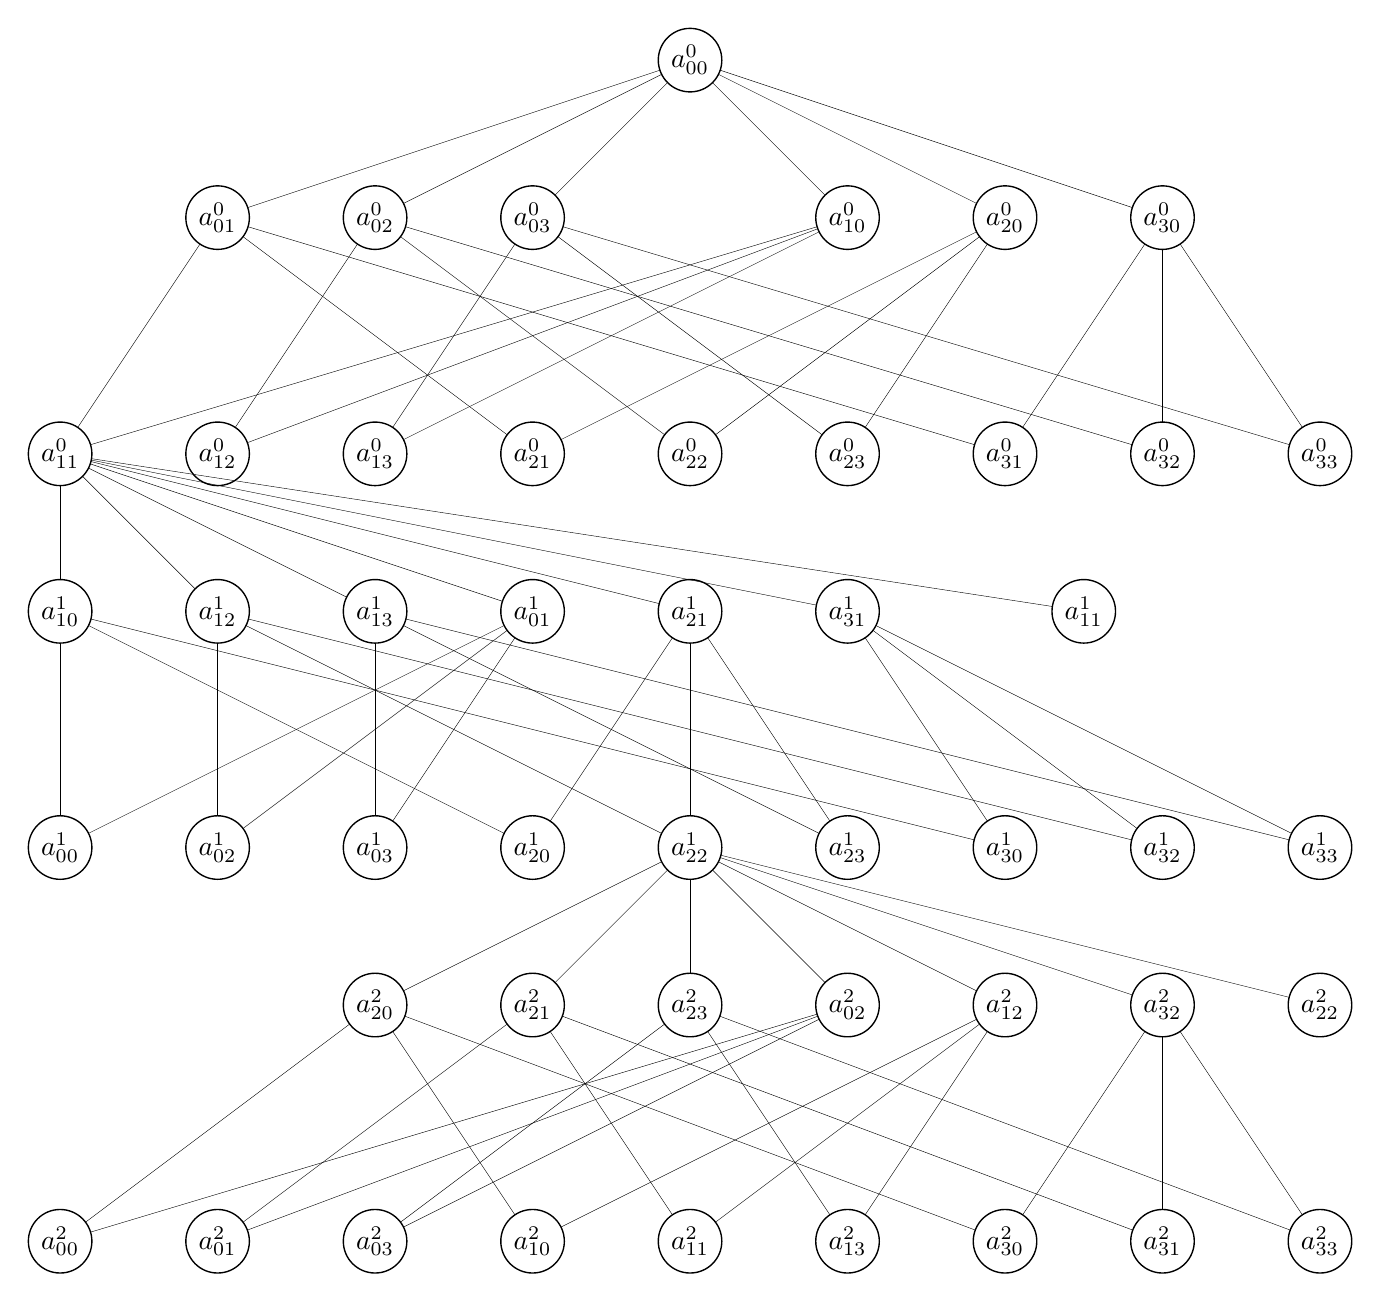
\begin{tikzpicture}

\Vertex[x=0, y=0, LabelOut=false]{$a_{00}^{0}$}
\Vertex[x=-6,y=-2]{$a_{01}^{0}$}
\Vertex[x=-4,y=-2]{$a_{02}^{0}$}
\Vertex[x=-2,y=-2]{$a_{03}^{0}$}
\Vertex[x=2,y=-2]{$a_{10}^{0}$}
\Vertex[x=4,y=-2]{$a_{20}^{0}$}
\Vertex[x=6,y=-2]{$a_{30}^{0}$}
\Edges($a_{00}^{0}$, $a_{01}^{0}$) 
\Edges($a_{00}^{0}$, $a_{02}^{0}$) 
\Edges($a_{00}^{0}$, $a_{03}^{0}$) 
\Edges($a_{00}^{0}$, $a_{10}^{0}$) 
\Edges($a_{00}^{0}$, $a_{20}^{0}$) 
\Edges($a_{00}^{0}$, $a_{30}^{0}$) 

\Vertex[x=-8,y=-5]{$a_{11}^{0}$}
\Vertex[x=-6,y=-5]{$a_{12}^{0}$}
\Vertex[x=-4,y=-5]{$a_{13}^{0}$}
\Vertex[x=-2,y=-5]{$a_{21}^{0}$}
\Vertex[x=0,y=-5]{$a_{22}^{0}$}
\Vertex[x=2,y=-5]{$a_{23}^{0}$}
\Vertex[x=4,y=-5]{$a_{31}^{0}$}
\Vertex[x=6,y=-5]{$a_{32}^{0}$}
\Vertex[x=8,y=-5]{$a_{33}^{0}$}
\Edges($a_{01}^{0}$, $a_{11}^{0}$, $a_{10}^{0}$) 
\Edges($a_{02}^{0}$, $a_{12}^{0}$, $a_{10}^{0}$) 
\Edges($a_{03}^{0}$, $a_{13}^{0}$, $a_{10}^{0}$) 
\Edges($a_{01}^{0}$, $a_{21}^{0}$, $a_{20}^{0}$) 
\Edges($a_{02}^{0}$, $a_{22}^{0}$, $a_{20}^{0}$) 
\Edges($a_{03}^{0}$, $a_{23}^{0}$, $a_{20}^{0}$) 
\Edges($a_{01}^{0}$, $a_{31}^{0}$, $a_{30}^{0}$) 
\Edges($a_{02}^{0}$, $a_{32}^{0}$, $a_{30}^{0}$) 
\Edges($a_{03}^{0}$, $a_{33}^{0}$, $a_{30}^{0}$) 

\Vertex[x=5,y=-7]{$a_{11}^{1}$}
\Edges($a_{11}^{0}$, $a_{11}^{1}$) 
\Vertex[x=-8,y=-7]{$a_{10}^{1}$}
\Vertex[x=-6,y=-7]{$a_{12}^{1}$}
\Vertex[x=-4,y=-7]{$a_{13}^{1}$}
\Vertex[x=-2,y=-7]{$a_{01}^{1}$}
\Vertex[x=0,y=-7]{$a_{21}^{1}$}
\Vertex[x=2,y=-7]{$a_{31}^{1}$}
\Edges($a_{11}^{0}$, $a_{10}^{1}$) 
\Edges($a_{11}^{0}$, $a_{12}^{1}$) 
\Edges($a_{11}^{0}$, $a_{13}^{1}$) 
\Edges($a_{11}^{0}$, $a_{01}^{1}$) 
\Edges($a_{11}^{0}$, $a_{21}^{1}$) 
\Edges($a_{11}^{0}$, $a_{31}^{1}$)

\Vertex[x=-8,y=-10]{$a_{00}^{1}$}
\Vertex[x=-6,y=-10]{$a_{02}^{1}$}
\Vertex[x=-4,y=-10]{$a_{03}^{1}$}
\Vertex[x=-2,y=-10]{$a_{20}^{1}$}
\Vertex[x=0,y=-10]{$a_{22}^{1}$}
\Vertex[x=2,y=-10]{$a_{23}^{1}$}
\Vertex[x=4,y=-10]{$a_{30}^{1}$}
\Vertex[x=6,y=-10]{$a_{32}^{1}$}
\Vertex[x=8,y=-10]{$a_{33}^{1}$}
\Edges($a_{01}^{1}$, $a_{00}^{1}$, $a_{10}^{1}$) 
\Edges($a_{12}^{1}$, $a_{02}^{1}$, $a_{01}^{1}$) 
\Edges($a_{13}^{1}$, $a_{03}^{1}$, $a_{01}^{1}$) 
\Edges($a_{10}^{1}$, $a_{20}^{1}$, $a_{21}^{1}$) 
\Edges($a_{12}^{1}$, $a_{22}^{1}$, $a_{21}^{1}$) 
\Edges($a_{21}^{1}$, $a_{23}^{1}$, $a_{13}^{1}$) 
\Edges($a_{10}^{1}$, $a_{30}^{1}$, $a_{31}^{1}$) 
\Edges($a_{12}^{1}$, $a_{32}^{1}$, $a_{31}^{1}$) 
\Edges($a_{13}^{1}$, $a_{33}^{1}$, $a_{31}^{1}$) 

\Vertex[x=8,y=-12]{$a_{22}^{2}$}
\Edges($a_{22}^{1}$, $a_{22}^{2}$) 
\Vertex[x=-4,y=-12]{$a_{20}^{2}$}
\Vertex[x=-2,y=-12]{$a_{21}^{2}$}
\Vertex[x=-0,y=-12]{$a_{23}^{2}$}
\Vertex[x=2,y=-12]{$a_{02}^{2}$}
\Vertex[x=4,y=-12]{$a_{12}^{2}$}
\Vertex[x=6,y=-12]{$a_{32}^{2}$}

\Edges($a_{22}^{1}$, $a_{20}^{2}$) 
\Edges($a_{22}^{1}$, $a_{21}^{2}$) 
\Edges($a_{22}^{1}$, $a_{23}^{2}$) 
\Edges($a_{22}^{1}$, $a_{02}^{2}$) 
\Edges($a_{22}^{1}$, $a_{12}^{2}$) 
\Edges($a_{22}^{1}$, $a_{32}^{2}$)

\Vertex[x=-8,y=-15]{$a_{00}^{2}$}
\Vertex[x=-6,y=-15]{$a_{01}^{2}$}
\Vertex[x=-4,y=-15]{$a_{03}^{2}$}
\Vertex[x=-2,y=-15]{$a_{10}^{2}$}
\Vertex[x=0,y=-15]{$a_{11}^{2}$}
\Vertex[x=2,y=-15]{$a_{13}^{2}$}
\Vertex[x=4,y=-15]{$a_{30}^{2}$}
\Vertex[x=6,y=-15]{$a_{31}^{2}$}
\Vertex[x=8,y=-15]{$a_{33}^{2}$}

\Edges($a_{20}^{2}$, $a_{00}^{2}$, $a_{02}^{2}$) 
\Edges($a_{21}^{2}$, $a_{01}^{2}$, $a_{02}^{2}$) 
\Edges($a_{23}^{2}$, $a_{03}^{2}$, $a_{02}^{2}$) 
\Edges($a_{20}^{2}$, $a_{10}^{2}$, $a_{12}^{2}$) 
\Edges($a_{21}^{2}$, $a_{11}^{2}$, $a_{12}^{2}$) 
\Edges($a_{23}^{2}$, $a_{13}^{2}$, $a_{12}^{2}$) 
\Edges($a_{20}^{2}$, $a_{30}^{2}$, $a_{32}^{2}$) 
\Edges($a_{21}^{2}$, $a_{31}^{2}$, $a_{32}^{2}$) 
\Edges($a_{23}^{2}$, $a_{33}^{2}$, $a_{32}^{2}$)
\end{tikzpicture}
\end{center}

\textbf{Σημείωση:} Προφανώς, στον παραπάνω γράφο, έχουμε άλλη μία επανάληψη που ξεκινάει από το $a_{33}^{2}$ για να υπολογιστούν οι τελικές τιμές και ακολουθεί το ίδιο μοτίβο.

\end{enumerate}


\subsubsection{Αναδρομική έκδοση}
Ο αναδρομικός αλγόριθμος είναι ο εξής:

\begin{lstlisting}[style=CStyle, mathescape]
FWR (A, B, C)
	if (base case)
		FWI (A, B, C)
	else
		FWR ($A_{11}, B_{11}, C_{11}$);
		FWR ($A_{12}, B_{11}, C_{12}$);
		FWR ($A_{21}, B_{21}, C_{11}$);
		FWR ($A_{22}, B_{21}, C_{12}$);
		FWR ($A_{22}, B_{21}, C_{12}$);
		FWR ($A_{21}, B_{21}, C_{11}$);
		FWR ($A_{12}, B_{11}, C_{12}$);
		FWR ($A_{11}, B_{11}, C_{11}$);


FWI (A, B, C)
	for (k=0; k<N; k++)
		for (i=0; i<N; i++)
			for (j=0; j<N; j++)
				A[i][j] = min(A[i][j], B[i][k]+C[k][j]); 
\end{lstlisting}

\begin{enumerate}
\item \textbf{Κατανομή Υπολογισμών}

Η συνάρτηση FWI θα κληθεί όταν οι πίνακες είναι αρκετά μικροί ώστε να χωρέσουν στην cache. Μπορούμε να θεωρήσουμε ως ένα task την εκτέλεση της συνάρτησης FWI, αλλά αρχικά για λόγους παρουσιάσης του task graph θεωρούμε ως task τον υπολογισμό της συνάρτησης FWR στο πρώτο επίπεδο της ανάδρομης. Αφού η λειτουργία είναι αναδρομική, ο γράφος επεκτείνεται αναδρομικά όπως θα δείξουμε παρακάτω.

\item \textbf{Ορισμός ορθής σειράς εκτέλεσης μέσω task graph}

Συμβολίζουμε ως $A_{i_1j_1}B_{i_2j_2}C_{i_3j_3}$ την κλήση της συνάρτηση FWR() στο 1ο επίπεδο της αναδρομής στα αντίστοιχα block του πίνακα, σύμφωνα μα το παρακάτω:

\begin{center}
 \begin{tabular}{|c  c | c  c|} 
 \hline
   \multicolumn{2}{|c|}{$A_{11}$} &    \multicolumn{2}{c|}{$A_{12}$} \\ 
   &&& \\
 \hline
   \multicolumn{2}{|c|}{$A_{21}$} &    \multicolumn{2}{c|}{$A_{22}$} \\ 
   &&& \\
 \hline
\end{tabular}
\end{center}

\begin{center}
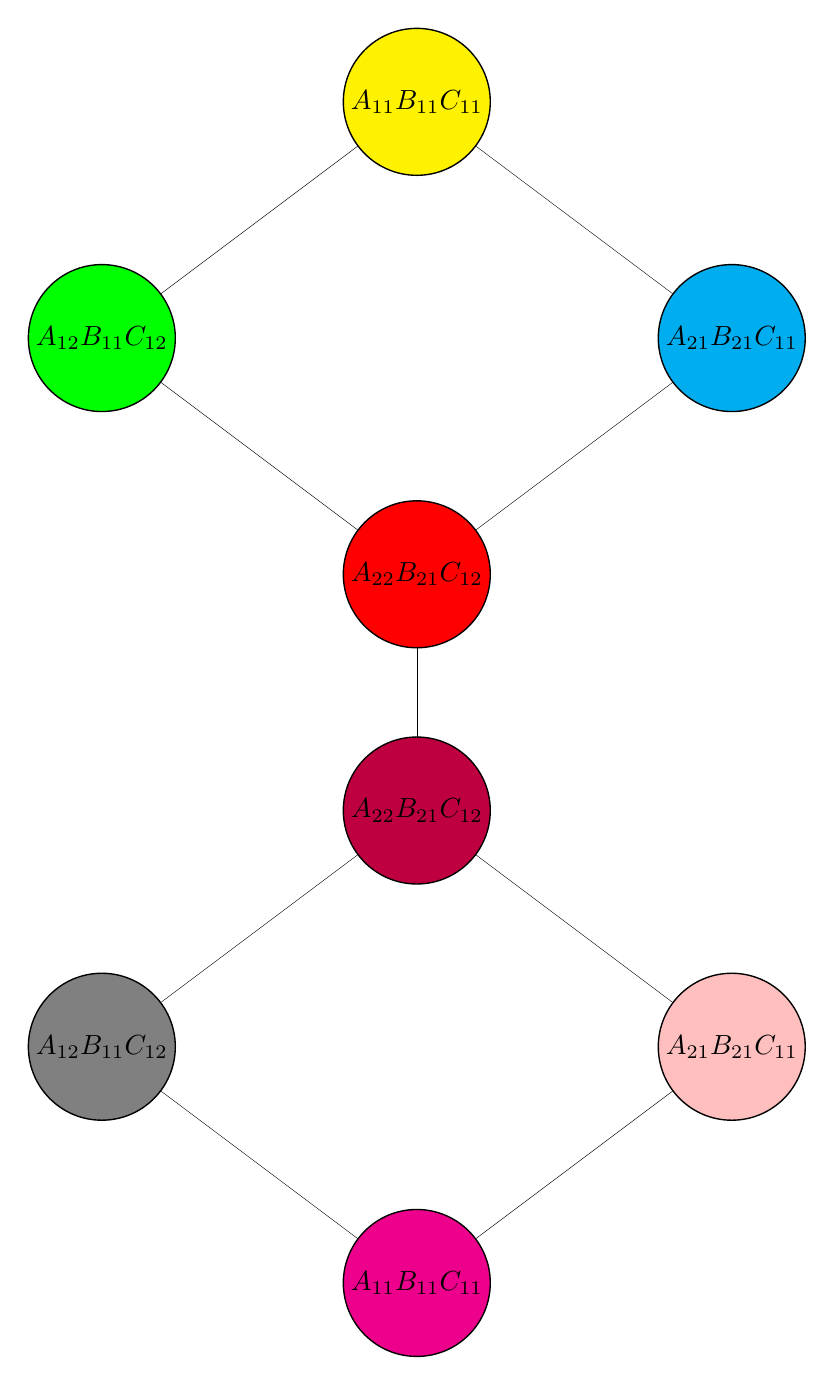
\begin{tikzpicture}

{\renewcommand{\VertexLightFillColor}{yellow}
\Vertex[x=0, y=0, LabelOut=false]{$A_{11} B_{11} C_{11}$}
}
{\renewcommand{\VertexLightFillColor}{green}
\Vertex[x=-4, y=-3, LabelOut=false]{$A_{12} B_{11} C_{12}$}
}
{\renewcommand{\VertexLightFillColor}{cyan}
\Vertex[x=4, y=-3, LabelOut=false]{$A_{21} B_{21} C_{11}$}
}
{\renewcommand{\VertexLightFillColor}{red}
\Vertex[x=0, y=-6, LabelOut=false]{$A_{22} B_{21} C_{12}$}
}
{\renewcommand{\VertexLightFillColor}{purple}
\Vertex[x=0, y=-9, LabelOut=false]{$A_{22} B_{21} C_{12} $}
}
{\renewcommand{\VertexLightFillColor}{pink}
\Vertex[x=4, y=-12, LabelOut=false]{$A_{21} B_{21} C_{11} $}
}
{\renewcommand{\VertexLightFillColor}{gray}
\Vertex[x=-4, y=-12, LabelOut=false]{$A_{12} B_{11} C_{12} $}
}
{\renewcommand{\VertexLightFillColor}{magenta}
\Vertex[x=0, y=-15, LabelOut=false]{$A_{11} B_{11} C_{11} $}
}

\Edges($A_{12} B_{11} C_{12}$, $A_{11} B_{11} C_{11}$, $A_{21} B_{21} C_{11}$) 
\Edges($A_{12} B_{11} C_{12}$, $A_{22} B_{21} C_{12}$, $A_{21} B_{21} C_{11}$) 
\Edges($A_{22} B_{21} C_{12} $, $A_{22} B_{21} C_{12}$) 
\Edges($A_{21} B_{21} C_{11} $,$A_{22} B_{21} C_{12} $,$A_{12} B_{11} C_{12} $) 
\Edges($A_{21} B_{21} C_{11} $,$A_{11} B_{11} C_{11} $,$A_{12} B_{11} C_{12} $) 

\end{tikzpicture}
\end{center}

Παρακάτω, γίνεται μία προσπάθεια να θεωρήσουμε ως task τον υπολογισμό της FWI στην περίπτωση όπου έχουμε 8 κόμβους και στην cache χωράει block 2×2, με αποτέλεσμα η αναδρομή να έχει τρία επίπεδα. Έχουμε δηλαδή τον παρακάτω πίνακα όπου κάθε $A_{ij}$ είναι ένα block 2×2. Έχει διατηρηθεί ο ίδιος χρωματικός κώδικας έτσι ώστε να γίνει αντιληπτό σε ποιο task του 1ου γράφου αντιστοιχούν τα tasks του δεύτερου. Παρουσιάζονται οι 4 πρώτες κλήσεις της αναδρομής.

\begin{center}
 \begin{tabular}{|c | c || c | c|} 
 \hline
  $A_{00}$ & $A_{01}$ & $A_{02}$ & $A_{03}$ \\
 \hline
 $A_{10}$ & $A_{11}$ & $A_{12}$ & $A_{13}$ \\
 \hline
 \hline
 $A_{20}$ & $A_{21}$ & $A_{22}$ & $A_{23}$ \\ 
 \hline
 $A_{30}$ & $A_{31}$ & $A_{32}$ & $A_{33}$ \\
 \hline
\end{tabular}
\end{center}

\begin{center}
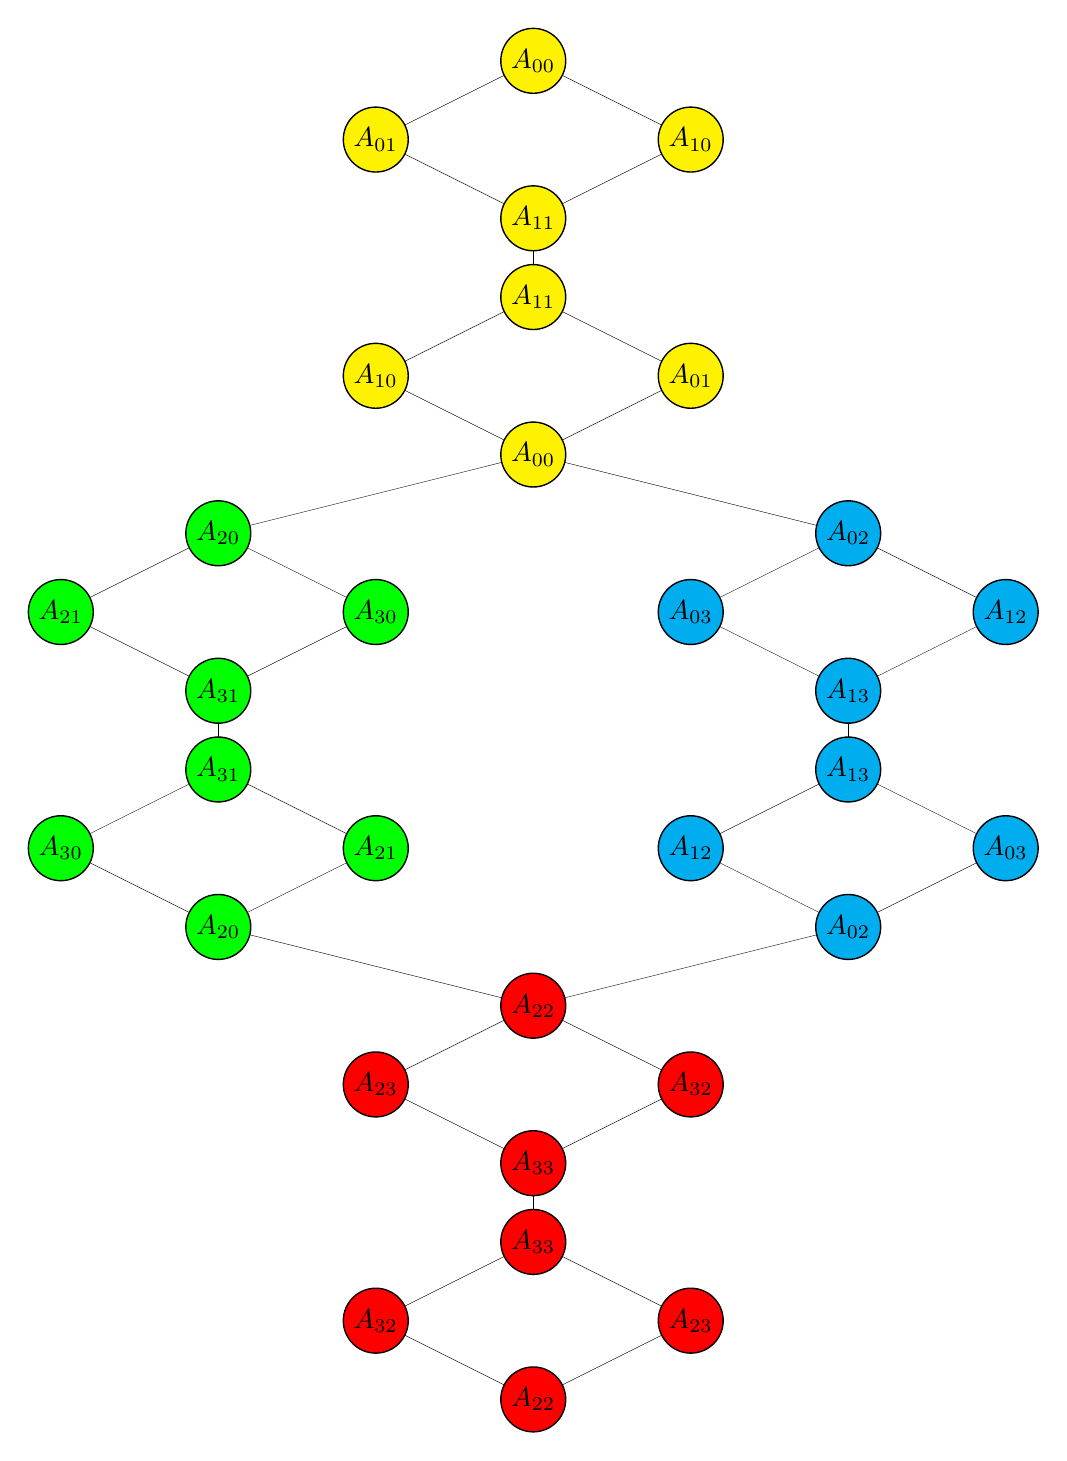
\begin{tikzpicture}

{\renewcommand{\VertexLightFillColor}{yellow}
\Vertex[x=0, y=0, LabelOut=false]{$A_{00}$}
\Vertex[x=-2, y=-1, LabelOut=false]{$A_{01}$}
\Vertex[x=2, y=-1, LabelOut=false]{$A_{10}$}
\Vertex[x=0, y=-2, LabelOut=false]{$A_{11}$}
\Vertex[x=0, y=-3, LabelOut=false]{$A_{11} $}
\Vertex[x=-2, y=-4, LabelOut=false]{$A_{10} $}
\Vertex[x=2, y=-4, LabelOut=false]{$A_{01} $}
\Vertex[x=0, y=-5, LabelOut=false]{$A_{00} $}

\Edges($A_{01}$, $A_{00}$, $A_{10}$) 
\Edges($A_{01}$, $A_{11}$, $A_{10}$) 
\Edges($A_{11} $, $A_{11}$) 
\Edges($A_{10} $,$A_{11} $,$A_{01} $) 
\Edges($A_{10} $,$A_{00} $,$A_{01} $) 
}

{\renewcommand{\VertexLightFillColor}{cyan}
\Vertex[x=4, y=-6, LabelOut=false]{$A_{02}$}
\Edges($A_{00} $, $A_{02}$) 
\Vertex[x=2, y=-7, LabelOut=false]{$A_{03}$}
\Vertex[x=6, y=-7, LabelOut=false]{$A_{12}$}
\Vertex[x=4, y=-8, LabelOut=false]{$A_{13}$}
\Vertex[x=4, y=-9, LabelOut=false]{$A_{13} $}
\Vertex[x=2, y=-10, LabelOut=false]{$A_{12} $}
\Vertex[x=6, y=-10, LabelOut=false]{$A_{03} $}
\Vertex[x=4, y=-11, LabelOut=false]{$A_{02} $}

\Edges($A_{03}$, $A_{02}$, $A_{12}$) 
\Edges($A_{03}$, $A_{13}$, $A_{12}$) 
\Edges($A_{13} $, $A_{13}$) 
\Edges($A_{12} $,$A_{13} $,$A_{03} $) 
\Edges($A_{12} $,$A_{02} $,$A_{03} $) 
}

{\renewcommand{\VertexLightFillColor}{green}
\Vertex[x=-4, y=-6, LabelOut=false]{$A_{20}$}
\Edges($A_{00} $, $A_{20}$) 
\Vertex[x=-6, y=-7, LabelOut=false]{$A_{21}$}
\Vertex[x=-2, y=-7, LabelOut=false]{$A_{30}$}
\Vertex[x=-4, y=-8, LabelOut=false]{$A_{31}$}
\Vertex[x=-4, y=-9, LabelOut=false]{$A_{31} $}
\Vertex[x=-6, y=-10, LabelOut=false]{$A_{30} $}
\Vertex[x=-2, y=-10, LabelOut=false]{$A_{21} $}
\Vertex[x=-4, y=-11, LabelOut=false]{$A_{20} $}

\Edges($A_{21}$, $A_{20}$, $A_{30}$) 
\Edges($A_{21}$, $A_{31}$, $A_{30}$) 
\Edges($A_{31} $, $A_{31}$) 
\Edges($A_{30} $,$A_{31} $,$A_{21} $) 
\Edges($A_{30} $,$A_{20} $,$A_{21} $) 
}

{\renewcommand{\VertexLightFillColor}{red}
\Vertex[x=0, y=-12, LabelOut=false]{$A_{22}$}
\Edges($A_{20} $, $A_{22}$) 
\Edges($A_{02} $, $A_{22}$)
\Vertex[x=-2, y=-13, LabelOut=false]{$A_{23}$}
\Vertex[x=2, y=-13, LabelOut=false]{$A_{32}$}
\Vertex[x=0, y=-14, LabelOut=false]{$A_{33}$}
\Vertex[x=0, y=-15, LabelOut=false]{$A_{33} $}
\Vertex[x=-2, y=-16, LabelOut=false]{$A_{32} $}
\Vertex[x=2, y=-16, LabelOut=false]{$A_{23} $}
\Vertex[x=0, y=-17, LabelOut=false]{$A_{22} $}

\Edges($A_{23}$, $A_{22}$, $A_{32}$) 
\Edges($A_{23}$, $A_{33}$, $A_{32}$) 
\Edges($A_{33} $, $A_{33}$) 
\Edges($A_{23} $,$A_{33} $,$A_{32} $) 
\Edges($A_{23} $,$A_{22} $,$A_{32} $) 
}
\end{tikzpicture}
\end{center}



\end{enumerate} 


\subsubsection{Tiled έκδοση}

Η tiled έκδοση του αλγορίθμου, αντίστοιχα με την recursive, στοχεύει στο να εφαρμόσει τον κλασσικό αλγόριθμο σε blocks του πίνακα (tiles εδώ). Έτσι, εφαρμόζει επαναληπτικά τις παρακάτω 3 φάσεις:

\begin{itemize}
\item Εφαρμογή FW στο tile $A_{kk}$
\item Εφαρμογή FW στα tiles $A_{ik}$ και $A_{ki}$ χρησιμοποιώντας το $A_{kk}$.
\item Εφαρμογή FW στα υπόλοιπα tiles $A_{ij}$ χρησιμοποιώντας κάθε φορά τα $A_{ik}$ και $A_{ki}$.
\end{itemize}

\begin{enumerate}
\item \textbf{Κατανομή Υπολογισμών}

Θεωρούμε ως ένα task την εφαρμογή του κλασσικού Floyd-Warshall αλγορίθμου σε ένα tile.

\item \textbf{Ορισμός ορθής σειράς εκτέλεσης μέσω task graph}

Παρουσιάζουμε το task graph για ένα πίνακα όπου $\frac{\boldsymbol{table \ size}}{\boldsymbol{tile \ size}} = 4$.
Συνεπώς, ο πίνακας των tiles είναι ο εξής:

\begin{center}
 \begin{tabular}{|c | c | c | c|} 
 \hline
  $A_{00}$ & $A_{01}$ & $A_{02}$ & $A_{03}$ \\
 \hline
 $A_{10}$ & $A_{11}$ & $A_{12}$ & $A_{13}$ \\
 \hline
 $A_{20}$ & $A_{21}$ & $A_{22}$ & $A_{23}$ \\ 
 \hline
 $A_{30}$ & $A_{31}$ & $A_{32}$ & $A_{33}$ \\
 \hline
\end{tabular}
\end{center}

\begin{center}
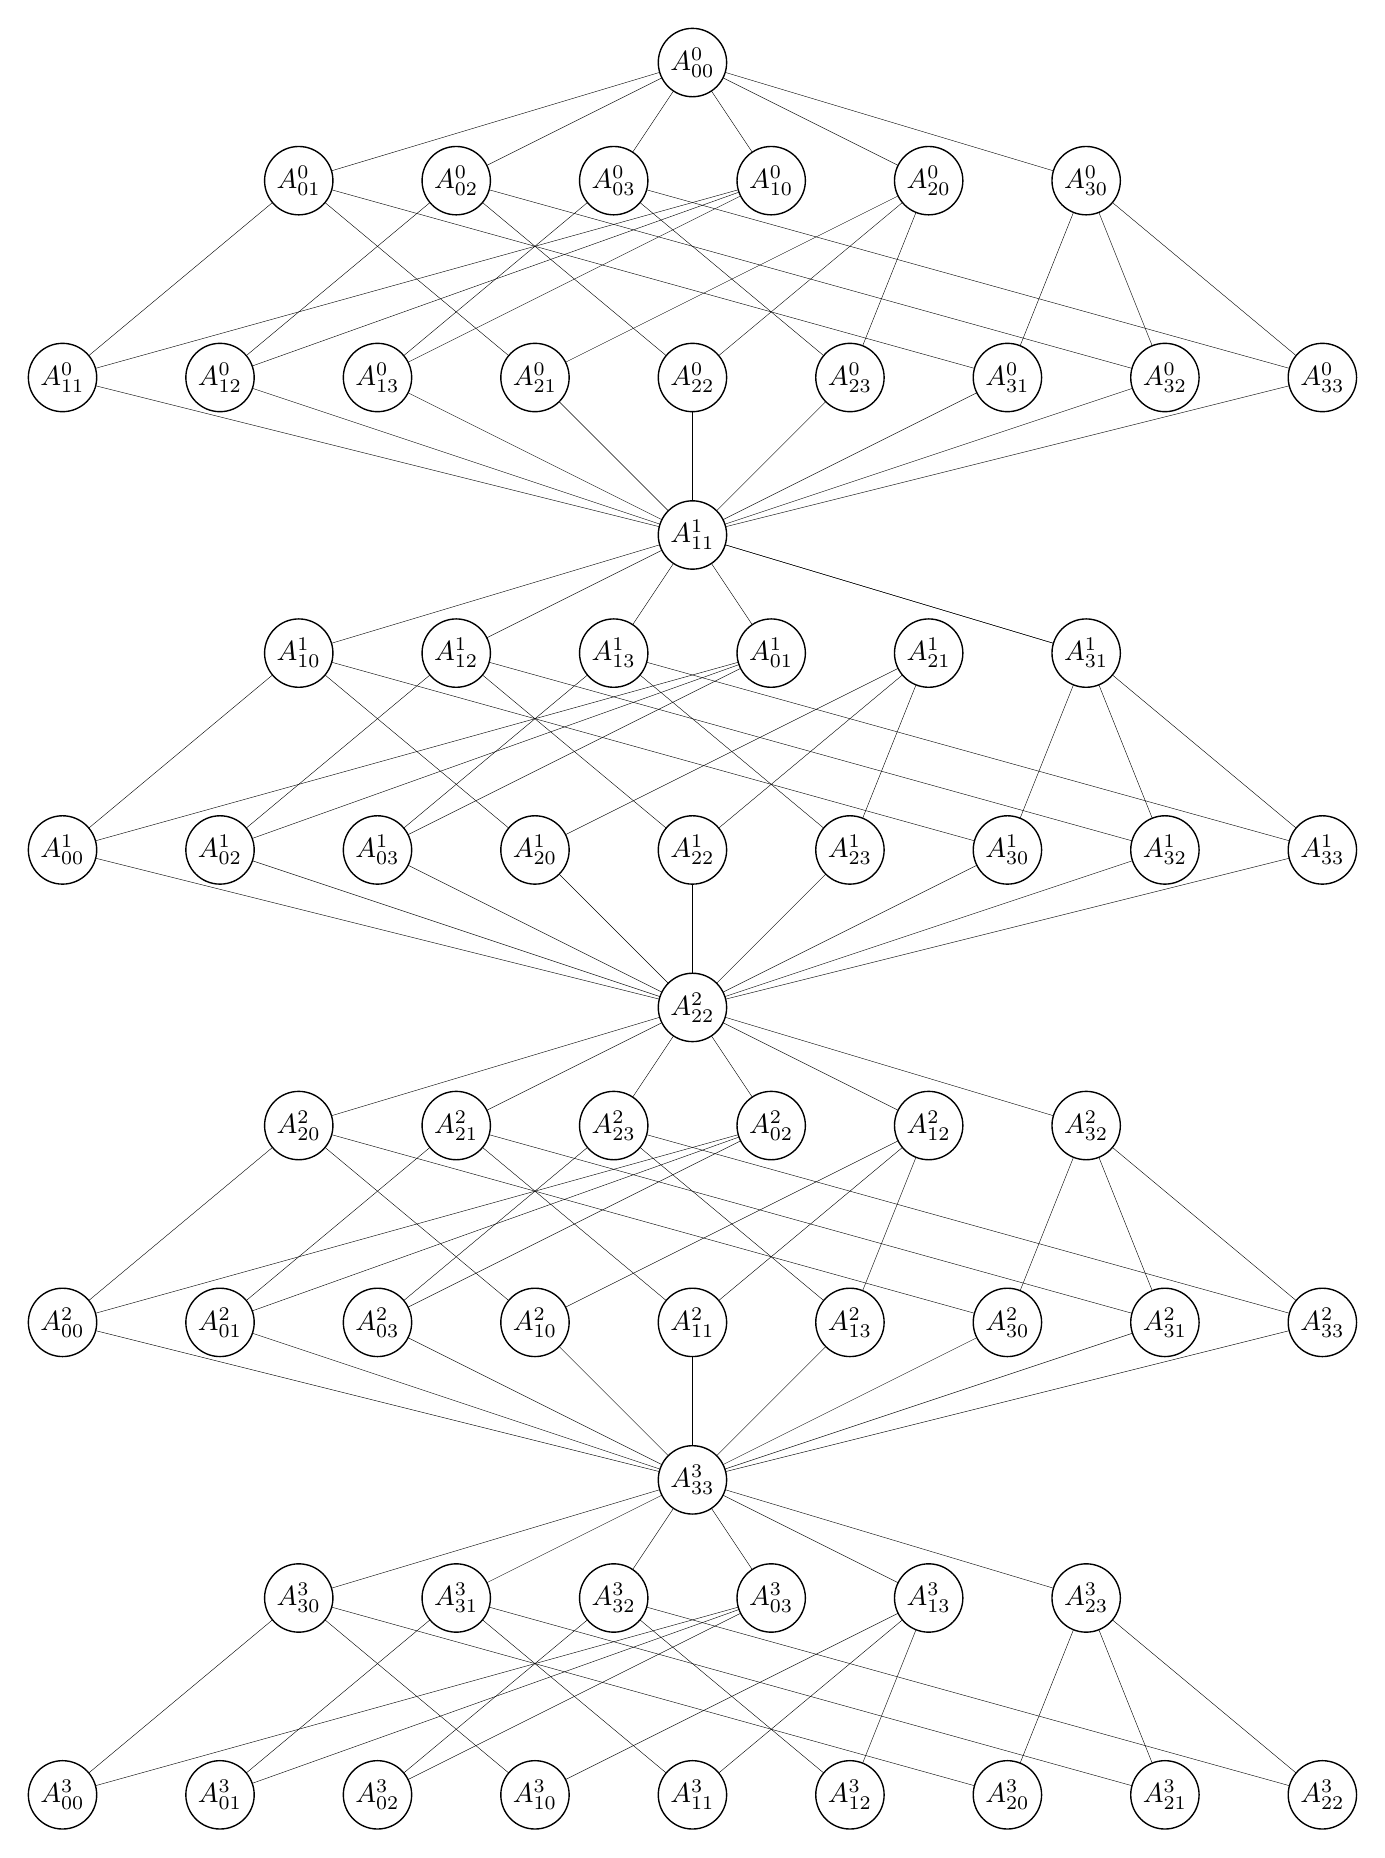
\begin{tikzpicture}

\Vertex[x=0, y=0, LabelOut=false]{$A_{00}^0$}

\Vertex[x=-5, y=-1.5, LabelOut=false]{$A_{01}^0$}
\Vertex[x=-3, y=-1.5, LabelOut=false]{$A_{02}^0$}
\Vertex[x=-1, y=-1.5, LabelOut=false]{$A_{03}^0$}

\Vertex[x=1, y=-1.5, LabelOut=false]{$A_{10}^0$}
\Vertex[x=3, y=-1.5, LabelOut=false]{$A_{20}^0$}
\Vertex[x=5, y=-1.5, LabelOut=false]{$A_{30}^0$}

\Edges($A_{01}^0$,$A_{00}^0$,$A_{02}^0$)
\Edges($A_{03}^0$,$A_{00}^0$,$A_{10}^0$) 
\Edges($A_{20}^0$,$A_{00}^0$,$A_{30}^0$) 

\Vertex[x=-8, y=-4, LabelOut=false]{$A_{11}^0$}
\Vertex[x=-6, y=-4, LabelOut=false]{$A_{12}^0$}
\Vertex[x=-4, y=-4, LabelOut=false]{$A_{13}^0$}

\Vertex[x=-2, y=-4, LabelOut=false]{$A_{21}^0$}
\Vertex[x=0, y=-4, LabelOut=false]{$A_{22}^0$}
\Vertex[x=2, y=-4, LabelOut=false]{$A_{23}^0$}

\Vertex[x=4, y=-4, LabelOut=false]{$A_{31}^0$}
\Vertex[x=6, y=-4, LabelOut=false]{$A_{32}^0$}
\Vertex[x=8, y=-4, LabelOut=false]{$A_{33}^0$}

\Edges($A_{01}^0$,$A_{11}^0$,$A_{10}^0$)
\Edges($A_{02}^0$,$A_{12}^0$,$A_{10}^0$) 
\Edges($A_{03}^0$,$A_{13}^0$,$A_{10}^0$) 

\Edges($A_{01}^0$,$A_{21}^0$,$A_{20}^0$)
\Edges($A_{02}^0$,$A_{22}^0$,$A_{20}^0$) 
\Edges($A_{03}^0$,$A_{23}^0$,$A_{20}^0$) 

\Edges($A_{01}^0$,$A_{31}^0$,$A_{30}^0$)
\Edges($A_{02}^0$,$A_{32}^0$,$A_{30}^0$) 
\Edges($A_{03}^0$,$A_{33}^0$,$A_{30}^0$) 

\Vertex[x=0, y=-6, LabelOut=false]{$A_{11}^1$}
\Edges($A_{11}^0$,$A_{11}^1$,$A_{12}^0$)
\Edges($A_{13}^0$,$A_{11}^1$,$A_{21}^0$) 
\Edges($A_{22}^0$,$A_{11}^1$,$A_{23}^0$) 
\Edges($A_{31}^0$,$A_{11}^1$,$A_{32}^0$) 
\Edges($A_{33}^0$,$A_{11}^1$) 

\Vertex[x=-5, y=-7.5, LabelOut=false]{$A_{10}^1$}
\Vertex[x=-3, y=-7.5, LabelOut=false]{$A_{12}^1$}
\Vertex[x=-1, y=-7.5, LabelOut=false]{$A_{13}^1$}

\Vertex[x=1, y=-7.5, LabelOut=false]{$A_{01}^1$}
\Vertex[x=3, y=-7.5, LabelOut=false]{$A_{21}^1$}
\Vertex[x=5, y=-7.5, LabelOut=false]{$A_{31}^1$}

\Edges($A_{10}^1$,$A_{11}^1$,$A_{12}^1$)
\Edges($A_{13}^1$,$A_{11}^1$,$A_{01}^1$) 
\Edges($A_{31}^1$,$A_{11}^1$,$A_{31}^1$) 

\Vertex[x=-8, y=-10, LabelOut=false]{$A_{00}^1$}
\Vertex[x=-6, y=-10, LabelOut=false]{$A_{02}^1$}
\Vertex[x=-4, y=-10, LabelOut=false]{$A_{03}^1$}

\Vertex[x=-2, y=-10, LabelOut=false]{$A_{20}^1$}
\Vertex[x=0, y=-10, LabelOut=false]{$A_{22}^1$}
\Vertex[x=2, y=-10, LabelOut=false]{$A_{23}^1$}

\Vertex[x=4, y=-10, LabelOut=false]{$A_{30}^1$}
\Vertex[x=6, y=-10, LabelOut=false]{$A_{32}^1$}
\Vertex[x=8, y=-10, LabelOut=false]{$A_{33}^1$}

\Edges($A_{10}^1$,$A_{00}^1$,$A_{01}^1$)
\Edges($A_{12}^1$,$A_{02}^1$,$A_{01}^1$) 
\Edges($A_{13}^1$,$A_{03}^1$,$A_{01}^1$) 

\Edges($A_{10}^1$,$A_{20}^1$,$A_{21}^1$)
\Edges($A_{12}^1$,$A_{22}^1$,$A_{21}^1$) 
\Edges($A_{13}^1$,$A_{23}^1$,$A_{21}^1$) 

\Edges($A_{10}^1$,$A_{30}^1$,$A_{31}^1$)
\Edges($A_{12}^1$,$A_{32}^1$,$A_{31}^1$) 
\Edges($A_{13}^1$,$A_{33}^1$,$A_{31}^1$) 

\Vertex[x=0, y=-12, LabelOut=false]{$A_{22}^2$}
\Edges($A_{00}^1$,$A_{22}^2$,$A_{02}^1$)
\Edges($A_{03}^1$,$A_{22}^2$,$A_{20}^1$) 
\Edges($A_{22}^1$,$A_{22}^2$,$A_{23}^1$) 
\Edges($A_{30}^1$,$A_{22}^2$,$A_{32}^1$) 
\Edges($A_{33}^1$,$A_{22}^2$) 

\Vertex[x=-5, y=-13.5, LabelOut=false]{$A_{20}^2$}
\Vertex[x=-3, y=-13.5, LabelOut=false]{$A_{21}^2$}
\Vertex[x=-1, y=-13.5, LabelOut=false]{$A_{23}^2$}

\Vertex[x=1, y=-13.5, LabelOut=false]{$A_{02}^2$}
\Vertex[x=3, y=-13.5, LabelOut=false]{$A_{12}^2$}
\Vertex[x=5, y=-13.5, LabelOut=false]{$A_{32}^2$}

\Edges($A_{20}^2$,$A_{22}^2$,$A_{21}^2$)
\Edges($A_{23}^2$,$A_{22}^2$,$A_{02}^2$) 
\Edges($A_{12}^2$,$A_{22}^2$,$A_{32}^2$) 

\Vertex[x=-8, y=-16, LabelOut=false]{$A_{00}^2$}
\Vertex[x=-6, y=-16, LabelOut=false]{$A_{01}^2$}
\Vertex[x=-4, y=-16, LabelOut=false]{$A_{03}^2$}

\Vertex[x=-2, y=-16, LabelOut=false]{$A_{10}^2$}
\Vertex[x=0, y=-16, LabelOut=false]{$A_{11}^2$}
\Vertex[x=2, y=-16, LabelOut=false]{$A_{13}^2$}

\Vertex[x=4, y=-16, LabelOut=false]{$A_{30}^2$}
\Vertex[x=6, y=-16, LabelOut=false]{$A_{31}^2$}
\Vertex[x=8, y=-16, LabelOut=false]{$A_{33}^2$}

\Edges($A_{20}^2$,$A_{00}^2$,$A_{02}^2$)
\Edges($A_{21}^2$,$A_{01}^2$,$A_{02}^2$) 
\Edges($A_{23}^2$,$A_{03}^2$,$A_{02}^2$) 

\Edges($A_{20}^2$,$A_{10}^2$,$A_{12}^2$)
\Edges($A_{21}^2$,$A_{11}^2$,$A_{12}^2$) 
\Edges($A_{23}^2$,$A_{13}^2$,$A_{12}^2$) 

\Edges($A_{20}^2$,$A_{30}^2$,$A_{32}^2$)
\Edges($A_{21}^2$,$A_{31}^2$,$A_{32}^2$) 
\Edges($A_{23}^2$,$A_{33}^2$,$A_{32}^2$) 

\Vertex[x=0, y=-18, LabelOut=false]{$A_{33}^3$}
\Edges($A_{00}^2$,$A_{33}^3$,$A_{01}^2$)
\Edges($A_{03}^2$,$A_{33}^3$,$A_{10}^2$) 
\Edges($A_{11}^2$,$A_{33}^3$,$A_{13}^2$) 
\Edges($A_{30}^2$,$A_{33}^3$,$A_{31}^2$) 
\Edges($A_{33}^2$,$A_{33}^3$)

\Vertex[x=-5, y=-19.5, LabelOut=false]{$A_{30}^3$}
\Vertex[x=-3, y=-19.5, LabelOut=false]{$A_{31}^3$}
\Vertex[x=-1, y=-19.5, LabelOut=false]{$A_{32}^3$}

\Vertex[x=1, y=-19.5, LabelOut=false]{$A_{03}^3$}
\Vertex[x=3, y=-19.5, LabelOut=false]{$A_{13}^3$}
\Vertex[x=5, y=-19.5, LabelOut=false]{$A_{23}^3$}

\Edges($A_{30}^3$,$A_{33}^3$,$A_{31}^3$)
\Edges($A_{32}^3$,$A_{33}^3$,$A_{03}^3$) 
\Edges($A_{13}^3$,$A_{33}^3$,$A_{23}^3$) 

\Vertex[x=-8, y=-22, LabelOut=false]{$A_{00}^3$}
\Vertex[x=-6, y=-22, LabelOut=false]{$A_{01}^3$}
\Vertex[x=-4, y=-22, LabelOut=false]{$A_{02}^3$}

\Vertex[x=-2, y=-22, LabelOut=false]{$A_{10}^3$}
\Vertex[x=0, y=-22, LabelOut=false]{$A_{11}^3$}
\Vertex[x=2, y=-22, LabelOut=false]{$A_{12}^3$}

\Vertex[x=4, y=-22, LabelOut=false]{$A_{20}^3$}
\Vertex[x=6, y=-22, LabelOut=false]{$A_{21}^3$}
\Vertex[x=8, y=-22, LabelOut=false]{$A_{22}^3$}

\Edges($A_{30}^3$,$A_{00}^3$,$A_{03}^3$)
\Edges($A_{31}^3$,$A_{01}^3$,$A_{03}^3$) 
\Edges($A_{32}^3$,$A_{02}^3$,$A_{03}^3$) 

\Edges($A_{30}^3$,$A_{10}^3$,$A_{13}^3$)
\Edges($A_{31}^3$,$A_{11}^3$,$A_{13}^3$) 
\Edges($A_{32}^3$,$A_{12}^3$,$A_{13}^3$) 

\Edges($A_{30}^3$,$A_{20}^3$,$A_{23}^3$)
\Edges($A_{31}^3$,$A_{21}^3$,$A_{23}^3$) 
\Edges($A_{32}^3$,$A_{22}^3$,$A_{23}^3$) 

\end{tikzpicture}
\end{center}




\end{enumerate}






\newpage
\nocite{notes}
\bibliography{sources} 
\bibliographystyle{ieeetr}

\end{document}